\documentclass{article}

\usepackage[greek,english]{babel}
\usepackage[utf8x]{inputenc}
\usepackage{natbib}
\usepackage{graphicx}
\usepackage{subfigure}
\graphicspath{ {.//} }
\usepackage{xcolor}
\graphicspath{ {./images/} }
\usepackage{titling}

\setlength{\droptitle}{10em}

\title{%
  \selectlanguage{greek}\Huge
 Μοντέλα υπολογιστικού νέφους \\}
  


\begin{document}
\selectlanguage{greek}

\author{\selectlanguage{greek}\LARGE
  Γεώργιος Νικολάου\\
   \texttt{\selectlanguage{english}\large sdi1800134}
  \and
  \selectlanguage{greek}\LARGE
  Νεφέλη Ταβουλάρη\\
   \texttt{\selectlanguage{english}\large sdi1800190}
}

\maketitle


\begin{figure}
\centering
\begin{subfigure}
  \centering
  
\includegraphics[width=40mm]{dit_logo}
  \label{fig:sub1}
\end{subfigure}%
\begin{subfigure}
  \centering
  
\includegraphics[width=50mm]{NKUA_logo}
  \label{fig:sub2}
\end{subfigure}
\label{fig:test}
\end{figure}




\newpage
\tableofcontents
\newpage
\section{Εισαγωγή}
\section{Σύγχρονα Πληροφοριακά Συστήματα}
\subsection{Ανάπτυξη}
\subsection{Νέες Ανάγκες}
\section{Υπολογιστικό Νέφος}
Με βάση τον ορισμό του\selectlanguage{english} NIST, \selectlanguage{greek}το Υπολογιστικό Νέφος έιναι ένα μοντέλο που επιτρέπει μια πανταχού παρούσα και με βάση τη ζήτηση \selectlanguage{english}(on demand, pay-per-use)\selectlanguage{greek} δικτυακή σύνδεση σε διαμοιρασμένους υπολογιστικούς πόρους (πχ δίκτυο, αποθήκευση, εφαρμογές, υπηρεσίες, σέρβερς), που μπορούν γρήγορα και εύκολα να υπολογιστούν και να διατεθούν από έναν πάροχο.
\subsection{Οφέλη}
\begin{itemize}
\item Ο καταναλωτής πληρώνει για όσα χρησιμοποιεί\selectlanguage{english} (pay-as-you-go),\selectlanguage{greek} δεν υποαπασχολεί πόρους, ούτε χρησιμοποιεί πόρους που δε χρειάζεται. Γι’ αυτό και παλιότερα το\selectlanguage{english} Cloud Computing \selectlanguage{greek}ονομαζόταν \selectlanguage{english}Utility Computing.\selectlanguage{greek}
\item Μετακινώντας τις εφαρμογές του στο Νέφος, απαλλάσσεται από τα έξοδα για την απόκτηση και τη συντήρηση εξοπλισμού.
\item Με διάφορες στρατηγικές \selectlanguage{english}(λag strategy, lead strategy, match strategy), \selectlanguage{greek}ο χρήστης έχει τη δυνατότητα να αυξομειώνει τις εικονικές μηχανές ή όποιον άλλο πόρο, είτε προληπτικά, είτε ύστερα από την υπέρβαση κάποιου ορίου/threshold, με αποτέλεσμα να είναι πάντα εξασφαλισμένος από άποψη μνήμης, επεξεργαστή κτλ, αλλά και να ελαχιστοποιεί το κόστος του. Μια εταιρεία, λοιπόν, στο Νέφος μπορεί να γίνει πιο προσαρμοστική στις αλλαγές\selectlanguage{english} (organizational agility).\selectlanguage{greek} Έτσι, επιτυγχάνεται κλιμάκωση \selectlanguage{english}(scalability, rapid elasticity), \selectlanguage{greek}δηλαδή αποδοτικότητα παρά την αύξηση του φόρτου.
\item Ενά από τα βασικότερα χαρακτηρηστικά του Νέφους είναι η εικονικοποίηση\selectlanguage{english} (virtualization), \selectlanguage{greek}με την οποία πολλά αντίγραφα ενός περιβάλλοντος σέρβερ (λειτουργικό σύστημα και εφαρμογές) μπορούν να φιλοξενηθούν σε ένα φυσικό σέρβερ, ο οποίος διαμοιράζεται. 
\item Αποφεύγεται το\selectlanguage{english} single point of failure\selectlanguage{greek} καθώς μια εφαρμογή «απλώνεται» σε πολλούς σέρβερς, που συχνά βρίσκονται και σε διαφορετικά γεωγραφικά σημεία\selectlanguage{english} (availability zones)\selectlanguage{greek}
\item Κορυφαίας Τεχνολογίας πόροι, και επιλεγμένοι για να ικανοποιούν τη συγκεκριμένη ανάγκη κάθε φορά
\item Ασφάλεια, προστασία από επιθέσεις, κρυπτογράφηση, αυθεντικοποίηση, απομόνωση δεδομένων χρηστών

\end{itemize}
















\subsection{Προκλήσεις}
\section{Μοντέλα υπολογιστικού νέφους}
Ο όρος «Ως Υπηρεσία» \selectlanguage{english}(as a Service), \selectlanguage{greek}αναφέρεται σε μια υπηρεσία Υπολογιστικού Νέφους, η οποία παρέχεται από ένα τρίτο μέρος, με σκοπό να μπορεί ο χρήστης να αφοσιωθεί σε ό,τι έχει περισσότερη σημασία για εκείνον, στην ανάπτυξη ισχυρών και χρήσιμων Πληροφοριακών Συστημάτων και την αύξηση της παραγωγικότητας ή του κέρδους. Ακολουθεί, λοιπόν, μια φιλοσοφία \selectlanguage{english}"Black Box",\selectlanguage{greek} η οποία διευκολύνει το χρήστη και ενθαρρύνει την καινοτομία και τον ανταγωνισμό.

\subsection{Λογισμικό ως Υπηρεσία - \selectlanguage{english}SaaS\selectlanguage{greek}}
Αναμφισβήτητα,η αγορά λογισμικού για τις επιχειρηματικές ανάγκες μιας εταιρείας αποτελεί μια κρίσιμη και περίπλοκη διαδικασία. Στόχος είναι πάντα η ελαχιστοποίηση του κόστους , αλλά και η αύξηση της παραγωγικότητας, επενδύοντας σε όσο μεγαλύτερους αυτοματισμούς. Συνηθισμένα παραδείγματα λογισμικού που χρησιμοποιούνται από τις επιχειρήσεις είναι τα εξής:
\begin{itemize}
  \item Λογισμικό εσωτερικής επικοινωνίας, πχ \selectlanguage{english} Microsoft Teams, Zoom, Webex, Outlook, Jira, Confluence, Slack\selectlanguage{greek}
  \item Λογισμικό για διαχείριση λογιστικών, φορολογικών διαδικασιών
  \item \selectlanguage{english} Enterprise Resource Planning programs (ERP)
  \item Office 365, \selectlanguage{greek}πχ \selectlanguage{english}Word, Excel, Access, Google Docs
  \item Portal \selectlanguage{greek} εταιρείας, διαχείριση αδειών, διαχείριση tickets στο \selectlanguage{english}ΙΤ \selectlanguage{greek}τμήμα \selectlanguage{english}
  \item Version Control System,\selectlanguage{greek} πχ \selectlanguage{english}Github, Gitlab, Bitbucket \selectlanguage{greek}
  \item Λογισμικό διαχείρισης Ανθρωπίνου Δυναμικού \selectlanguage{english}
  \item Customer Relationship Management (CRP), Marketing programs
  \item CAD \selectlanguage{greek}Λογισμικό\selectlanguage{english}
  \item Code Editor,\selectlanguage{greek} πχ\selectlanguage{english} VSCode, IntelliJ, PyCharm\selectlanguage{greek}

\end{itemize}
Παραδοσιακά, αυτή η ανάγκη των εταιρειών ικανοποιούνταν με το λεγόμενο, Λογισμικό ως Προϊόν \selectlanguage{english}(Software as a Product, SaaP), \selectlanguage{greek}βάσει του οποίου, η εταιρεία αγοράζει άδεια για να χρησιμοποιεί τη συγκεκριμένη υπηρεσία, την οποία φιλοξενεί ύστερα, στις εγκαταστάσεις της \selectlanguage{english}(on premises).\selectlanguage{greek} Επίσης, αναλαμβάνει τα έξοδα συντήρησης και ανανέωσης του λογισμικού. \\ \\
Ωστόσο, με την ανάπτυξη του Υπολογιστικού Νέφους, το Λογισμικό ως Υπηρεσία γίνεται όλο και πιο διαδεδομένο.Το Λογισμικό ως Υπηρεσία, γνωστό και ως \selectlanguage{english}Software as a Service (SaaS) \selectlanguage{greek}αναφέρεται στην παροχή ενός λογισμικού / πληροφοριακού συστήματος, το οποίο φιλοξενείται κεντρικά, στο Νέφος. Η φιλοσοφία πίσω από αυτή τη μέθοδο, είναι πως ο χρήστης μπορεί να απολαμβάνει μια ηλεκτρονική υπηρεσία, χωρίς να χρειάζεται να διαχειρίζεται τις υποδομές, το δίκτυο, τις βάσεις δεδομένων, το ενδιάμεσο λογισμικό, τους διακομιστές / σέρβερς, τα δεδομένα, το λειτουργικό σύστημα, αλλά ούτε και τις εφαρμογές. Εν ολίγοις, ο χρήστης χρησιμοποιεί το Πληροφοριακό Σύστημα , ως συνδρομητής, για να ικανοποιήσει τις ανάγκες του και ο Πάροχος της υπηρεσίας αναλαμβάνει να διαχειρίζεται όλους τους απαιτούμενους πόρους για να λειτουργεί σωστά η εφαρμογή.  \\ 
Τα κυριότερα πλεονεκτήματα ενός τέτοιου μοντέλου είναι τα εξής :
\begin{itemize}
    \itemΧαμηλότερο κόστος για τις επιχειρήσεις και τους ιδιώτες, οι οποίοι δε χρειάζεται να αγοράσουν το λογισμικό και τις απαραίτητες άδειες. Ανάπτυξη οικονομίας κλίμακας με μείωση κόστους συντήρησης και παροχής του λογισμικού. Επίσης, το κόστος είναι συγκεκριμένο \selectlanguage{english}(pay-as-you-go) \selectlanguage{greek}και πολλές φορές δεν υπάρχει από την αρχή της χρήσης (πχ \selectlanguage{english}Netflix).\selectlanguage{greek} 
    \itemΔεν υπάρχει ανάγκη γνώσης χρήσης των διαφόρων λογισμικών, ούτε επομένως και εξειδικευμένου προσωπικού\selectlanguage{english}  (expertise) \selectlanguage{greek} σε μια επιχείρηση, με αποτέλεσμα ξανά τη μείωση κόστους. Ευχρηστία, σύνδεση στην εφαρμογή μέσω κάποιου \selectlanguage{english}Dashboard\selectlanguage{greek} ή \selectlanguage{english}API.\selectlanguage{greek}
    \itemΠρόσβαση από παντού, μέσω Διαδικτύου και οποιασδήποτε συσκευής, χωρίς να χρειάζεται να εγκατασταθεί πρόσθετο λογισμικό (πχ \selectlanguage{english}dependencies,\selectlanguage{greek} εργαλεία, packages, λειτουργικό σύστημα), ή σύνδεση με \selectlanguage{english}VPN\selectlanguage{greek}. Επιτυγχάνεται, λοιπόν, μεγαλύτερη ευελιξία και αύξηση της παραγωγικότητας 
    \itemΌλοι οι χρήστες έχουν την ίδια έκδοση, η οποία αναβαθμίζεται αυτόματα
    \itemΠρόκειται για ολοκληρωμένα και εύχρηστα Πληροφοριακά Συστήματα, ανεξάρτητα από το Λειτουργικό Σύστημα ή το Υλικό του καθενός, ακολουθούν επομένως τις αρχές της εικονικοποίησης (\selectlanguage{english}virtualization)\selectlanguage{greek} και της αφαιρετικότητας (\selectlanguage{english}abstraction)\selectlanguage{greek}
    \itemΚαλύτερη συνεργασία μέσα σε μια εταιρεία, λόγω του \selectlanguage{english}multitenancy,\selectlanguage{greek} δηλαδή της παράλληλης χρήσης της ίδιας εφαρμογής από πολλούς χρήστες. Χαρακτηριστικό του \selectlanguage{english}Multitenancy\selectlanguage{greek} είναι πως οι χρήστες νιώθουν σα να έχουν αποκλειστική χρήση του Λογισμικού
    \itemΑσφάλεια από κακόβουλους εισβολείς, προστασία, απόδοση, προσβασιμότητα, υψηλή διαθεσιμότητα, κλιμάκωση, αξιοπιστία και γενικότερα, όλα τα γνωστά πλεονεκτήματα του\selectlanguage{english} Cloud Computing\selectlanguage{greek}. Καθώς οι διάφορες εφαρμογές φιλοξενούνται σε κορυφαία \selectlanguage{english}Data Centers,\selectlanguage{greek} ειδικά σχεδιασμένα με αυτό το σκοπό, σε υψηλού επιπέδου υποδομές, με \selectlanguage{english}firewalls,\selectlanguage{greek} κρυπτογράφηση και ελεγχόμενη πρόσβαση
    \itemΧρησιμοποιώντας \selectlanguage{english}SaaS, \selectlanguage{greek}μια επιχείρηση έχει την ευκαιρία να αφοσιωθεί σε αυτό που την ενδιαφέρει πιο πολύ, το προϊόν της. Το ίδιο βέβαια ισχύει και για τους ιδιώτες. Αύξηση, λοιπόν, της καινοτομίας και της ευκινησίας \selectlanguage{english}(agility)
\selectlanguage{greek}
\end{itemize}

Τα κυριότερα μειονεκτήματα του μοντέλου:
\begin{itemize}
 \itemΑναγκαία η χρήση Διαδικτύου, διαφορετικά δεν μπορεί να υπάρξει πρόσβαση στην εφαρμογή
\itemΧαμηλή ασφάλεια ευαίσθητων δεδομένων, αν δεν είναι έμπιστος ο πάροχος
\itemΈλλειψη ελέγχου, καθώς η υπηρεσία είναι έτοιμη για χρήση και δεν είναι εύκολο να μεταβληθεί και να προσαρμοστεί στις ανάγκες του κάθε χρήστη
\itemΧαμηλή ταχύτητα μετάδοσης της εφαρμογής, καθώς ο σέρβερ μπορεί να βρίσκεται σε μεγάλη απόσταση από το \selectlanguage{english}Browser, \selectlanguage{greek}όπου τη χρησιμοποιεί ο χρήστης. Για αυτό είναι αναγκαία η επένδυση σε γρήγορη ταχύτητα Διαδικτύου
\item Δυσκολία συμμόρφωσης με τους κανονισμούς της κυβέρνησης για τα προσωπικά δεδομένα. Η κάθε επιχείρηση θα πρέπει να ενημερωθεί κατάλληλα για τις υποχρεώσεις της.
\end{itemize}
Συμπέρασμα : \\ \\
Με τη σωστή επιλογή ενός γνωστού και αποδεκτού παρόχου υπηρεσιών λογισμικού, την υπογραφή Συμφωνητικού για το Επίπεδο Λειτουργίας Υπηρεσίας,\selectlanguage{english} SLA (service level agreement),\selectlanguage{greek} όπου καταγράφονται όλες οι νομικές υποχρεώσεις του παρόχου, καθώς και με τη χρήση\selectlanguage{english}  5G,\selectlanguage{greek} το Λογισμικό ως Υπηρεσία είναι μια φτηνή και σίγουρη επιλογή για μια επιχείρηση, ειδικά αν δεν αναζητά κάποια εξειδικευμένη υπηρεσία, όπου έχει ανάγκη\selectlanguage{english}  customization.\selectlanguage{greek}


\subsection{Πλατφόρμα ως Υπηρεσία - \selectlanguage{english}PaaS\selectlanguage{greek}}
Το μοντέλο Πλατφόρμα ως Υπηρεσία \selectlanguage{english}(PaaS)\selectlanguage{greek} επιτρέπει στους χρήστες να επωφελούνται από τις υποδομές, το δίκτυο, το λειτουργικό σύστημα, τις βάσεις δεδομένων, τα οποία διαχειρίζεται και συντηρεί ο πάροχος της υπηρεσίας και ταυτόχρονα να έχουν την ευελιξία να σχεδιάσουν και να υλοποιήσουν ο,τιδήποτε επιθυμούν για την επιχείρησή τους, χρησιμοποιώντας έτοιμες μικρο-υπηρεσίες που υπάρχουν ήδη στο περιβάλλον της πλατφόρμας. Διατίθεται μέσω \selectlanguage{english} public, private \selectlanguage{greek}και \selectlanguage{english}hybrid\selectlanguage{greek} νέφους. \\
Παραδείγματα της Πλατφόρμας ως Υπηρεσία :
\begin{itemize}
\item Πλατφόρμα Επικοινωνίας ως Υπηρεσία, \selectlanguage{english}Communications Platform as a Service    (CPaaS) \selectlanguage{greek},η οποία περιλαμβάνει συνδυασμό ήχου, βίντεο, μηνυμάτων, πχ \selectlanguage{english}Skype, WhatsApp
\item Mobile Platform as a Service, \selectlanguage{greek}για την εύκολη ανάπτυξη εφαρμογών \selectlanguage{english}(Integrated Development Environment, IDE)
\item Open PaaS, open source / \selectlanguage{greek}ανοιχτού κώδικα πλατφόρμα, όπου ο χρήστης μπορεί να αναπτύξει εφαρμογές, πολλές φορές με οποιαδήποτε γλώσσα προγραμματισμού ή βάση δεδομένων επιθυμεί πχ \selectlanguage{english}Google App Engine, Microsoft Azure, Heroku\selectlanguage{greek}
\itemΜια άλλη αξιοσημείωτη χρήση \selectlanguage{english}PaaS \selectlanguage{greek}είναι στα \selectlanguage{english}DevOps tools (CI/CD pipelines), Agile Development
\item Integrations PaaS (iPaas) \selectlanguage{greek}για συγχώνευση δεδομένων, υπηρεσιών κτλ
\item \selectlanguage{english}AIPaaS, \selectlanguage{greek}για δημιουργία μοντέλων Μηχανικής Μάθησης με προεκπαιδευμένο/\selectlanguage{english}pre-trained\selectlanguage{greek} μοντέλα, τα οποία διευκολύνουν κατά πολύ τη διαδικασία 
\end{itemize}
Τα κυριότερα πλεονεκτήματα ενός τέτοιου μοντέλου είναι τα εξής :
\begin{itemize}
\item Οι προγραμματιστές μπορούν να αφοσιωθούν στην ανάπτυξη λογισμικού και συγκεκριμένα στη λογική \selectlanguage{english}(business intelligence)\selectlanguage{greek} πίσω από την εκάστοτε εφαρμογή, αντί να χάνουν χρόνο με την υποδομή, το δίκτυο, το λειτουργικό σύστημα, την αποθήκευση, τους διακομιστές. Όλα αυτά τα αναλαμβάνει ο πάροχος. Μείωση, λοιπόν, του \selectlanguage{english}low level programming,\selectlanguage{greek} το οποίο είναι και το πιο απαιτητικό.
\item Απλό μοντέλο, χαμηλό κόστος για ανάπτυξη εφαρμογών ,\selectlanguage{english} pay-as-you-go\selectlanguage{greek}
\item Προσβασιμότητα, υψηλή διαθεσιμότητα, κλιμάκωση
\item Μείωση απαιτούμενου κώδικα, καθώς παρέχονται έτοιμα πολλά χρήσιμα εργαλεία \selectlanguage{english}(pre-coded components, sample code, software tools, kits, libraries), \selectlanguage{greek}αύξηση της παραγωγικότητας 
\item Εύκολη μεταφορά στο Υβριδικό Νέφος
\item Έτοιμο περιβάλλον για \selectlanguage{english}versioning, build (debugger, compiler, code editor), deployment, testing, monitoring,\selectlanguage{greek} διαθέσιμα\selectlanguage{english} plugins\selectlanguage{greek} και \selectlanguage{english}frameworks\selectlanguage{greek} που διευκολύνουν αισθητά τη χρήση της πλατφόρμας. Επιπρόσθετα,  το μοντέλο \selectlanguage{english}PaaS \selectlanguage{greek}παρέχει συχνά εργαλεία για\selectlanguage{english} Data Analytics, \selectlanguage{greek}για δεδομένα που αφορούν το χρήστη ως προς την εφαρμογή.
\item Παροχή ενσωματωμένης βάσης \selectlanguage{english}(Database as a Service, \selectlanguage{greek}πχ \selectlanguage{english}MongoDB Atlas)\selectlanguage{greek},και γενικότερα έτοιμων και εύχρηστων υπηρεσιών
\item Παρέχει τα θετικά του \selectlanguage{english}SaaS, \selectlanguage{greek}όσον αφορά την ανεξαρτησία από τις υποδομές, αλλά προσφέρει ακόμη και επιπλέον ευελιξία, καθώς ο χρήστης μπορεί να δημιουργήσει ο,τιδήποτε επιθυμεί για να καλύψει πλήρως τις ανάγκες του, κάτι που ίσως δε θα μπορούσε να γίνει με ένα\selectlanguage{english} SaaS,\selectlanguage{greek} το οποίο δίνεται έτοιμο 
\item Παρόμοιο μοντέλο με το Συνάρτηση ως Υπηρεσία\selectlanguage{english} (Function as a Service), Serverless as a Service,\selectlanguage{greek} όπου σημασία έχει η λογική και όχι και η υποδομή
\end{itemize}
Τα κυριότερα μειονεκτήματα του μοντέλου:
\begin{itemize}
\item Δύσκολη μετακίνηση σε άλλο πάροχο, καθώς είναι πιθανό εκεί να γίνονται με άλλον τρόπο οι διαδικασίες ή να μην παρέχονται οι ίδιες υπηρεσίες/ευκολίες κτλ
\item Εξάρτηση από τον πάροχο, η τιμή μπορεί να αυξηθεί ανά πάσα στιγμή, αν υπάρξει πρόβλημα στις υποδομές, η εφαρμογή θα καταρρεύσει
\item Έλλειψη ελέγχου, όπως και στο μοντέλο Λογισμικό ως Υπηρεσία, καθώς κάποιος άλλος καθορίζει μεγάλο μέρος των \selectlanguage{english}configurations
\end{itemize}
\selectlanguage{greek}
Συμπέρασμα: \\ \\
Με τη σωστή επιλογή της υπηρεσίας, ώστε να καλύπτει τις ανάγκες της επιχείρησης/του χρήστη, αλλά και να ανήκει σε έμπιστο πάροχο, η Πλατφόρμα ως Υπηρεσία μπορεί να βελτιώσει και να διευκολύνει τη δουλειά του Developer, καθώς δε χρειάζεται να ξεκινάει από το μηδέν για κάθε του εργασία.

\subsection{Υποδομή ως Υπηρεσία -\selectlanguage{english} IaaS\selectlanguage{greek}}
Πρόκειται για ένα μοντέλο με το οποίο ο χρήστης/η επιχείρηση ενοικιάζεται και διαχειρίζεται, παρακολουθεί, αυξομειώνει πόρους \selectlanguage{english}(resources)\selectlanguage{greek}, μνήμη,\selectlanguage{english} CPU, \selectlanguage{greek}σέρβερς, βάσεις δεδομένων \selectlanguage{english}(replicas),\selectlanguage{greek} δικτυακό εξοπλισμό, τα οποία δε βρίσκονται στις τοπικές εγκαταστάσεις \selectlanguage{english}(on premises),\selectlanguage{greek} αλλά φιλοξενούνται στο\selectlanguage{english} cloud, \selectlanguage{greek}δηλαδή σε κάποιο \selectlanguage{english}Data Center.\selectlanguage{greek} Το όφελος αυτού του μοντέλου, και συνεπώς και των προαναφερθέντων, είναι ασύλληπτο, και οικονομικά αλλά και από άποψη χρόνου, προσπάθειας και ασφάλειας. \\ \\
Τα πιο γνωστά παραδείγματα \selectlanguage{english}IaaS:
\begin{itemize}
\item AWS (Amazon Web Services) EC2, 
\item Microsoft Azure, 
\item Google Cloud Platform, 
\item IBM Cloud, 
\item Oracle Cloud
\end{itemize}
\selectlanguage{greek}
Συγκεκριμένα τα πλεονεκτήματα είναι τα εξής : 

\begin{itemize}

\item Eλαχιστοποιείται το κόστος της κτήσης και συντήρησης της υλικοτεχνικής υποδομής \selectlanguage{english}(hardware),\selectlanguage{greek} μέσω της εικονικοποιήσης \selectlanguage{english}(virtualization), \selectlanguage{greek}διότι δεν υπάρχει ανάγκη για αγορά νέου εξοπλισμού. Ακόμα και για μια μικρή \selectlanguage{english}start-up\selectlanguage{greek} εταιρεία υπάρχει συμφέρον στη μεταφορά στο Νέφος.
\item Μπορεί εύκολα να επιτευχθεί κλιμάκωση και υψηλή διαθεσιμότητα\selectlanguage{english}(high availability), \selectlanguage{greek}μέσω διάφορων μεθόδων που συμφωνούνται στο\selectlanguage{english} SLA.\selectlanguage{greek} Έτσι, αν πχ τεθεί ένα όριο/threshold που αφορά την χρήση των πόρων, και το υπερβούμε, τότε αυτόματα και χωρίς καθυστέρηση θα μπουν σε χρήση νέοι πόροι. Επιπλέον, αν χρειαζόμαστε λιγότερους πόρους  απ’ ότι χρησιμοποιούσαμε μέχρι τώρα, μπορούμε πάλι εύκολα να κάνουμε \selectlanguage{english}scale down/in, \selectlanguage{greek}και να μειώσουμε το κόστος. Διαφορετικά, αν αυτές οι ενέργειες γίνοταν στις εγκαταστάσεις της εταιρείας, οι σέρβερς που είχαμε αγοράσει, θα έμεναν άπραγοι.
\item Λόγω του\selectlanguage{english} load balancing \selectlanguage{greek}που γίνεται με μικρό κόστος, αποφεύγεται το \selectlanguage{english}single point of failure,\selectlanguage{greek} δηλαδή η περίπτωση, αν κάτι δε δουλέψει σωστά, να καταρρεύσει όλη η εφαρμογή. Στο Νέφος, η εφαρμογή, τα δεδομένα, οι βάσεις δεδομένων βρίσκονται ταυτόχρονα σε πολλά σημεία, ακόμα και γεωγραφικά, ώστε να μην υπάρχει κανένας φόβος για τέτοιο ενδεχόμενο \selectlanguage{english}(availability zones).\selectlanguage{greek}
Στο \selectlanguage{english}IaaS, \selectlanguage{greek}λοιπόν, οι πόροι χρησιμοποιούνται ανάλογα με τη ζήτηση \selectlanguage{english}(on demand).\selectlanguage{greek}
\item Το \selectlanguage{english}IaaS \selectlanguage{greek}προσφέρει ασφάλεια, καθώς οι χρήστες που έχουν πρόσβαση στους διακομιστές κτλ φιλτράρονται.
\item Προσβασιμότητα από παντού, μέσω \selectlanguage{english}Web 2.0\selectlanguage{greek}
\item Λόγω της δύναμης των παρόχων στην αγορά, οι υποδομές που διατίθενται είναι κορυφαίας τεχνολογίας αλλά και επιλεγμένες για την κάθε ξεχωριστή περίπτωση και για τις ανάγκες του κάθε πελάτη. Επίσης, καθιστούν δυνατή την επεξεργασία \selectlanguage{english}Big Data, \selectlanguage{greek}κάτι που προφανώς είναι απαραίτητο στη σύγχρονη εποχή
\item Το πιο ευέλικτο μοντέλο, ο χρήστης έχει πλήρη έλεγχο πάνω στις υποδομές\selectlanguage{english} (abstraction)\selectlanguage{greek}
\item Πολλοί χρήστες χρησιμοποιούν το ίδιο \selectlanguage{english}hardware (multitenancy)\selectlanguage{greek}
\item Μια επιχείρηση μπορεί να έχει πρόσβαση σε σέρβερς που βρίσκονται γεωγραφικά κοντά στους χρήστες της εφαρμογής, με αποτέλεσμα να μεταδίδεται με καλύτερη ταχύτητα το προϊόν.
\end{itemize}
 Τα κυριότερα μειονεκτήματα του μοντέλου:
\begin{itemize}
\item Πάντα υπάρχει η ανησυχία για την ασφάλεια των δεδομένων, ειδικά λόγω του\selectlanguage{english} multitenancy. \selectlanguage{greek}Πρέπει κανείς να σιγουρευτεί πως τα δεδομένα του είναι απομονωμένα από τους άλλους χρήστες
\item Αν κάποιος δε ξέρει να χειρίζεται σωστά τις υπηρεσίες του \selectlanguage{english}Cloud Provider,\selectlanguage{greek} υπάρχει ο κίνδυνος να κάνει λάθη που να του κοστίσουν ακριβά, ενώ στην περίπτωση πχ του\selectlanguage{english} SaaS \selectlanguage{greek}δεν υπάρχει αυτός ο κίνδυνος.
\end{itemize}
Ένα παρόμοιο και αξιοσημείωτο μοντέλο υπηρεσίας είναι το\selectlanguage{english} Bare-Metal as a Service (BMaaS),\selectlanguage{greek} με το οποίο ο χρήστης έχει άμεση πρόσβαση στο υλικό πίσω από την εφαρμογή του, και όχι σε μια εικονοποιημένη μορφή του, με αποτέλεσμα να έχει καλύτερο έλεγχο αλλά να του κοστίζει σε χρόνο. \\ \\
Συμπέρασμα: \\ \\
Όταν μια εταιρεία περιμένει μεγάλη ανάπτυξη, την οποία και δε μπορεί να προβλέψει ακριβώς, θα επωφεληθεί ιδιαιτέρως από τέτοιου είδους αυτοματισμούς στο υλικό.Ωστόσο, είναι σημαντικό για μια εταιρεία να έχει εξειδικευμένο προσωπικό που να ξέρει να παρακολουθεί τη χρήση των πόρων \selectlanguage{english}(monitoring), \selectlanguage{greek}να συμβουλεύεται\selectlanguage{english} Cloud Solutions Architects,\selectlanguage{greek} ώστε να χρησιμοποιεί πάντα τις πιο αποδοτικές υπηρεσίες, να παρακολουθεί το \selectlanguage{english}billing \selectlanguage{greek}και να θέτει\selectlanguage{english} thresholds \selectlanguage{greek}και\selectlanguage{english} alerts, \selectlanguage{greek}για να αποφύγει παραβιάσεις στην κατανάλωση των πόρων.

\section{Από το \selectlanguage{english}IaaS \selectlanguage{greek}στο \selectlanguage{english}SaaS}
Στην ουσία, δεν υπάρχει καλύτερο και χειρότερο μοντέλο, το ερώτημα είναι ποιο είναι το καλύτερο μοντέλο για τις ανάγκες μας. Κατά τη διάρκεια της μελέτης μας, ήταν εύκολο να παρατηρήσουμε πως προχωρώντας από το \selectlanguage{english}IaaS \selectlanguage{greek}στο \selectlanguage{english}SaaS,\selectlanguage{greek} το \selectlanguage{english}abstraction \selectlanguage{greek}και η ευκολία χρήσης αυξάνονται, αλλά ταυτόχρονα μειώνεται η ευελιξία, η ελευθερία και ο έλεγχος του χρήστη στην εφαρμογή. Οπότε με το μοντέλο Υποδομή ως Υπηρεσία, ο χρήστης έχει μεγαλύτερες ευθύνες και υποχρεώσεις ,καθώς ο πάροχος αναλαμβάνει μόνο το Υλικό μέρος που απαιτείται από την εφαρμογή. Η λογική και η υλοποίηση εξαρτώνται από το χρήστη. Αντίθετα, με το μοντέλο Λογισμικό ως Υπηρεσία, ο χρήστης απλά χρησιμοποιεί μια έτοιμη εφαρμογή, την οποία έχει αναπτύξει και συντηρεί αποκλειστικά ο πάροχος. Σε αυτή την περίπτωση όμως, δεν είναι πάντα εύκολο για το χρήστη να προσαρμόσει την εφαρμογή στις ανάγκες το. Οπότε μπορεί να μη τον ικανοποιεί. Το μοντέλο Πλατφόρμα ως Υπηρεσία είναι ανάμεσα στα δύο άλλα μοντέλα, όσον αφορά την ευελιξία, αλλά και την ευκολία χρήσης. Στην ουσία αποτελεί έναν εύκολο τρόπο για έναν προγραμματιστή να αναπτύξει ποιοτικές εφαρμογές, χωρίς να χρειάζεται να επανεφεύρει τον τροχό.

Το παρακάτω διάγραμμα ανακεφαλαιώνει όλα όσα αναφέραμε, αποδεικνύοντας τη σημασία του Υπολογιστικού Νέφους. 


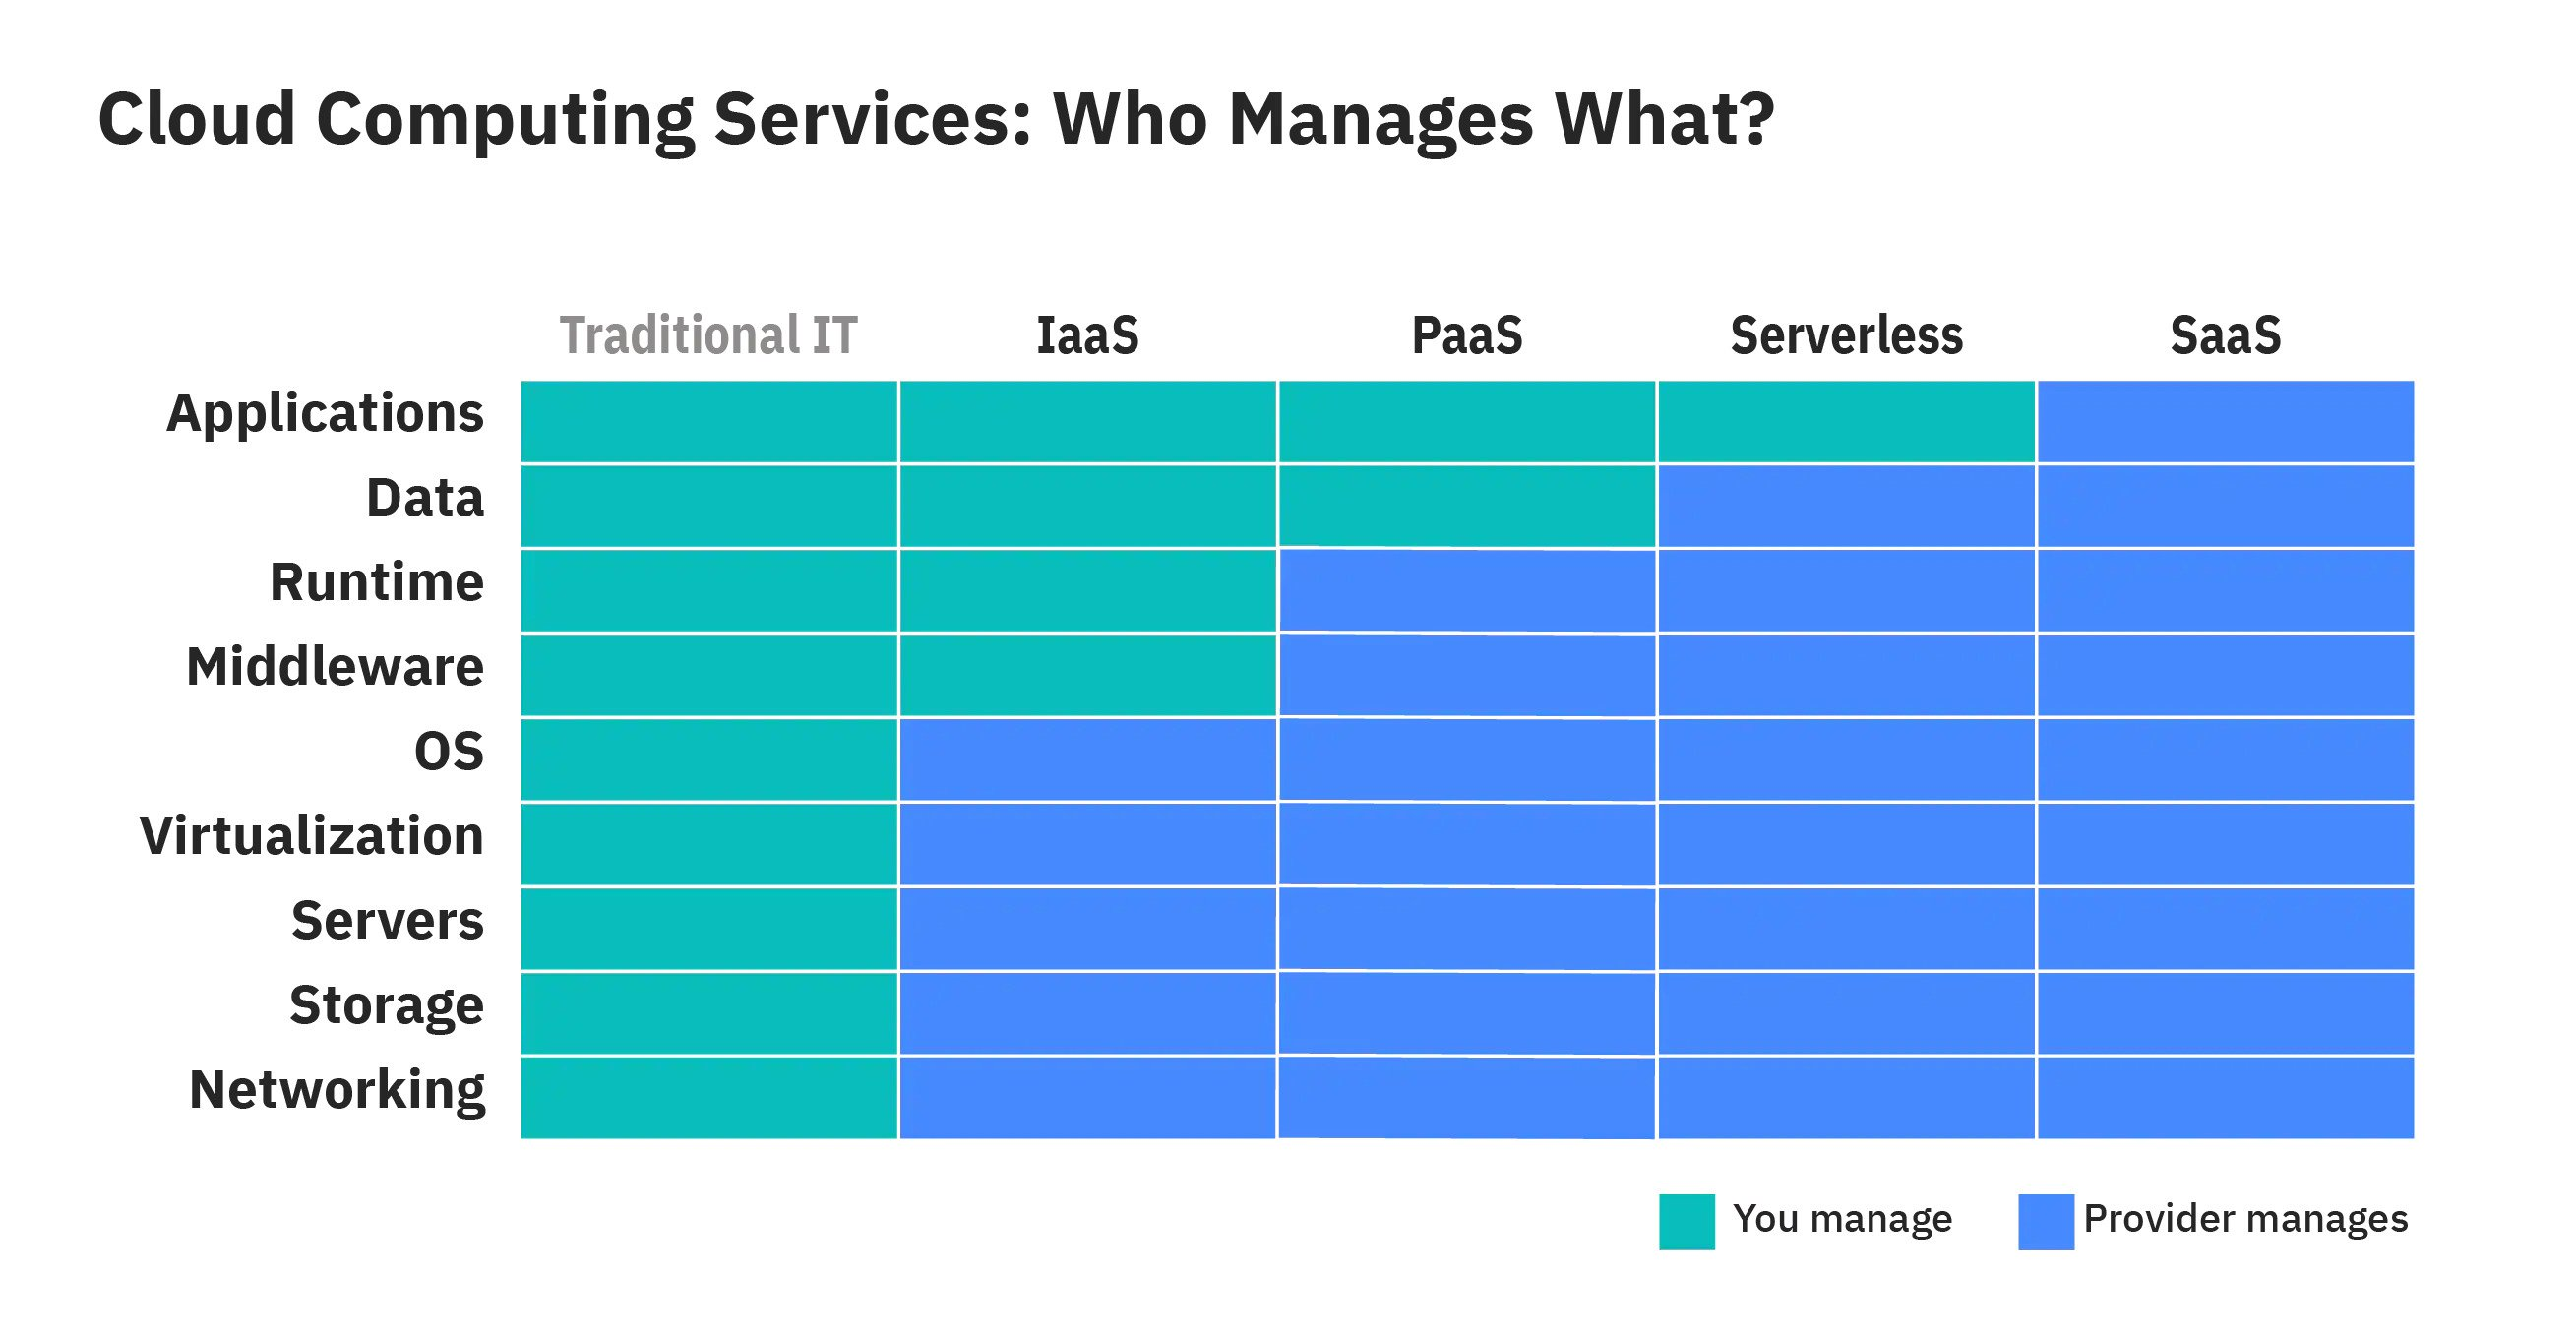
\includegraphics[width=120mm]{ibm.jpg}
Το συμπέρασμα από αυτή τη μελέτη όσον αφορά για τον αντίκτυπο του Νέφους στην κοινωνία:
\begin{itemize}
\item Μεγάλες και μικρομεσαίες επιχειρήσεις μπορούν να μετατρέψουν τις ιδέες τους σε επιχειρηματικά αποτελέσματα, πιο γρήγορα και χωρίς υπερβολικό κόστος.
\item Οι προγραμματιστές μπορούν να αφοσιωθούν στη επιχειρηματική λογική, αντί να ασχολούνται με περίπλοκες διαδικασίες που αφορούν τη διαχείριση του Υλικού.
\item	Οι απλοί χρήστες μπορούν να έχουν πρόσβαση στις διάφορες εφαρμογές από οποιαδήποτε συσκευή και να απολαμβάνουν άπειρες χρήσιμες υπηρεσίες
\end{itemize}

\section{Συμπεράσματα - Επισημάνσεις}
\end{document}
